\documentclass{article}
\usepackage[utf8x]{inputenc}
\usepackage[frenchb]{babel}
\usepackage[T1]{fontenc}
\usepackage{lmodern}
\usepackage{fullpage}
\usepackage{graphicx}
\usepackage{epstopdf}
\usepackage{caption}
\usepackage{subcaption}
\usepackage{multirow}
% Math symbols
\usepackage{amsmath}
\usepackage{amssymb}
\usepackage{amsthm}
% Numbers and units
\usepackage[squaren, Gray]{SIunits}
\usepackage{sistyle}
\usepackage{hyperref}
%\usepackage[autolanguage]{numprint}
%\usepackage{numprint}
\newcommand\si[2]{\numprint[#2]{#1}}
\newcommand\np[1]{\numprint{#1}}
\usepackage{enumitem}
%\usepackage{enumerate}

\DeclareMathOperator{\pgcd}{pgcd} % use \dif instead

\DeclareMathOperator{\newdiff}{d} % use \dif instead
\newcommand{\dif}{\newdiff\!}
\newcommand{\fpart}[2]{\frac{\partial #1}{\partial #2}}
\newcommand{\ffpart}[2]{\frac{\partial^2 #1}{\partial #2^2}}
\newcommand{\fdpart}[3]{\frac{\partial^2 #1}{\partial #2\partial #3}}
\newcommand{\fdif}[2]{\frac{\dif #1}{\dif #2}}
\newcommand{\ffdif}[2]{\frac{\dif^2 #1}{\dif #2^2}}
\newcommand{\constant}{\ensuremath{\mathrm{cst}}}
\newcommand{\bigoh}{\ensuremath{\mathcal{O}}}

% cfr http://en.wikibooks.org/wiki/LaTeX/Colors
\usepackage{color}
\usepackage[usenames,dvipsnames,svgnames,table]{xcolor}
\definecolor{dkgreen}{rgb}{0.25,0.7,0.35}
\definecolor{dkred}{rgb}{0.7,0,0}

\usepackage{listings}
\lstset{
  numbers=left,
  numberstyle=\tiny\color{gray},
  basicstyle=\rm\small\ttfamily,
  keywordstyle=\bfseries\color{dkred},
  frame=single,
  commentstyle=\color{gray}=small,
  stringstyle=\color{dkgreen},
  %backgroundcolor=\color{gray!10},
  %tabsize=2,
  rulecolor=\color{black!30},
  %title=\lstname,
  breaklines=true,
  framextopmargin=2pt,
  framexbottommargin=2pt,
  extendedchars=true,
  inputencoding=utf8x
}
\lstset{language={matlab}}

\title{}
\author{}

\newcommand{\I}{\mathcal{I}}
\newcommand{\lmax}{\lambda_\mathrm{max}}
\newcommand{\lmin}{\lambda_\mathrm{min}}

\usepackage{listings}
\usepackage{color}
\usepackage{textcomp}
\definecolor{listinggray}{gray}{0.9}
\definecolor{lbcolor}{rgb}{0.9,0.9,0.9}

%Pour insertion de codes matlab...
\lstset{
	backgroundcolor=\color{lbcolor},
numbers=left,
%
	tabsize=4,
	rulecolor=,
	language=matlab,
        basicstyle=\scriptsize,
        upquote=true,
        aboveskip={1.5\baselineskip},
        columns=fixed,
        showstringspaces=false,
        extendedchars=true,
        breaklines=true,
        prebreak = \raisebox{0ex}[0ex][0ex]{\ensuremath{\hookleftarrow}},
        frame=single,
        showtabs=false,
        showspaces=false,
        showstringspaces=false,
        identifierstyle=\ttfamily,
        keywordstyle=\color[rgb]{0,0,1},
        commentstyle=\color[rgb]{0.133,0.545,0.133},
        stringstyle=\color[rgb]{0.627,0.126,0.941},
}

\usepackage{algorithm}
\usepackage[noend]{algpseudocode}
\makeatletter
\def\BState{\State\hskip-\ALG@thistlm}
\makeatother

\begin{document}
\begin{titlepage}
\newcommand{\HRule}{\rule{\linewidth}{0.5mm}} % Defines a new command for the horizontal lines, change thickness here
\centering % Center everything on the page
 
%	HEADING SECTIONS
\null
\vspace{1cm}
\textsc{\Large Université Catholique de Louvain}\\[1cm] % Name of your university/college
\textsc{\large MECA2170 \\[0.3cm] Numerical Geometry}\\[0.5cm] % Major heading such as course name
%\textsc{\large Minor Heading}\\[0.5cm] % Minor heading such as course title

%	TITLE SECTION

\HRule \\[0.4cm]
{ \LARGE \bfseries Delaunay's triangulation\\[0.4cm] % Title of your document
\large \bfseries Report} \\[0.4cm]

\HRule \\[0.5cm]
 
\begin{figure}[!h]
	\begin{center}
	%2048 × 1364
		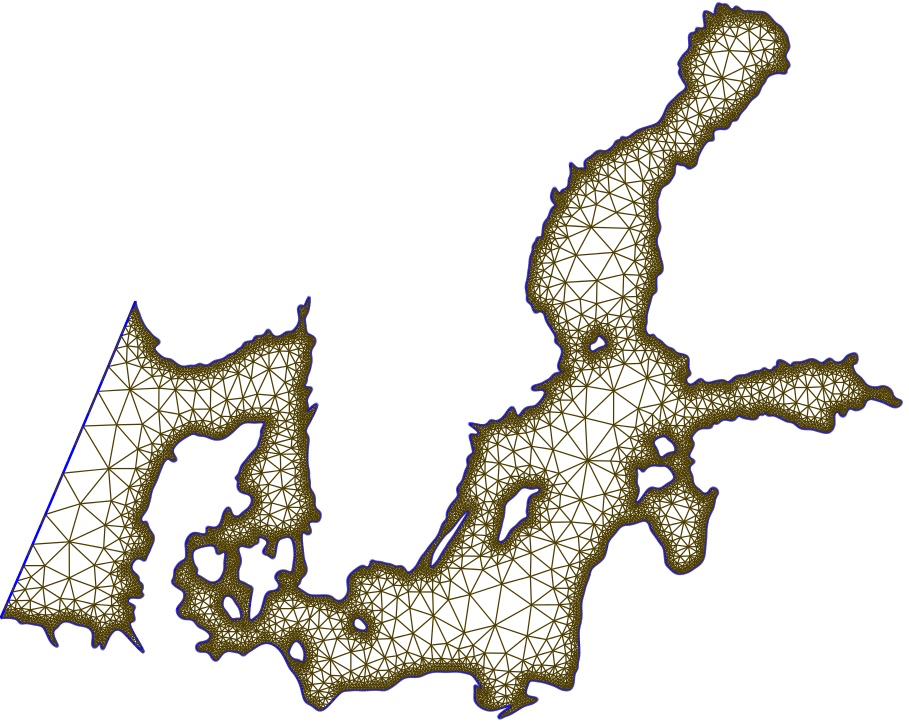
\includegraphics[width=10.5cm]{images/cover.jpg}
	\end{center}
\end{figure}

%	AUTHOR SECTION

\large 
\centering
{\begin{tabular}{lll}
\textsc{CERCKEL} & Arnaud\\
\textsc{STEVENS} & Nicolas\\
\end{tabular}}
\\[1cm]

\normalsize
{\begin{tabular}{ll}
\textit{Professeurs} : & Vincent Legat \& Jean François Remacle\\
\end{tabular}}
\\[1cm]

%	DATE SECTION

{\normalsize \today}\\[2cm] % Date, change the \today to a set date if you want to be precise

\end{titlepage}
\newpage
\section*{Abstract}
This report studies the Delaunay's triangulation, more explicitly the Watson's algorithm. We first present the the whole algorithm and the data structure related to it. Then we have a deep insight in the robustness question. Finally we present the performance results of our code. 


\section{Delaunay's triangulation : Watson's algorithm}
Watson's algorithm \cite{de2000computational} is a randomized incremental algorithm, we add point by point maintaining the Delaunay's properties at each step. The input is an array of points containing the $x$ and $y$ coordinate of each point. The output is a file containing the $n$ triangles (this is $n$ lines and $3$ column containing indices of the nodes).

\subsection*{Data's structures}
We have seven data's structures.

\subsection*{Watson's algorithm}

\begin{algorithm}
\caption{Watson-DelaunayTriangulation($\mathcal{P}$)}\label{Delaunay}
\begin{algorithmic}[1]
\State \textit{Input} A set of $n$ points $\mathcal{P}$
\State \textit{Output} An array of Delaunay's triangles
\State Initialise the "big triangle" by choosing three extreme points 
\State Initialise the data's structures (the location tree $\mathcal{T}$ and the stack $\mathcal{S}$)
\State perform a random permutation on $\mathcal{P}$
\For {$r \gets 1$ \textbf{to} $n$}
\State Find triangle $p_ip_jp_k \in \mathcal{T}$ containing $p_r$
\If {$p_r$ lies in the interior of triangle $p_ip_jp_k$} 
\State Add edges from $p_r$ to $p_i$, $p_j$ and $p_k$ and create three new triangles. Add them to the structure $\mathcal{T}$ and actualise $\mathcal{S}$.
\State Legalize edge ($p_r$, $\overline{p_ip_j}$,triangle $p_ip_jp_r$,$\mathcal{S}$)
\State Legalize edge ($p_r$, $\overline{p_jp_k}$,triangle $p_rp_jp_k$,$\mathcal{S}$)
\State Legalize edge ($p_r$, $\overline{p_kp_i}$,triangle $p_ip_rp_k$,$\mathcal{S}$)
\Else ($p_r$ lies on an edge of triangle $p_ip_jp_k$, say $p_ip_j$)
\State Add edges from $p_r$ to $p_k$ and to $p_l$ (the opposite node in the adjacent triangle $p_ip_jp_l$) and create four new triangles. Add them to $\mathcal{T}$ and actualise $\mathcal{S}$.
\State Legalize edge ($p_r$, $\overline{p_ip_l}$,triangle $p_ip_rp_l$,$\mathcal{S}$)
\State Legalize edge ($p_r$, $\overline{p_lp_j}$,triangle $p_rp_jp_l$,$\mathcal{S}$)
\State Legalize edge ($p_r$, $\overline{p_jp_k}$,triangle $p_rp_jp_k$,$\mathcal{S}$)
\State Legalize edge ($p_r$, $\overline{p_kp_i}$,triangle $p_ip_rp_k$,$\mathcal{S}$)
\EndIf
\EndFor
\Return $\mathcal{S}$
\end{algorithmic}
\end{algorithm}

\begin{algorithm}
\caption{Legalize Edge($p_r$, $\overline{p_ip_j}$, triangle $p_ip_jp_r$,$\mathcal{S}$)} \label{legalizeEdge}
\begin{algorithmic}[1]
\State Let $p_ip_jp_k$ be the adjacent triangle to $p_ip_jp_r$. Test if $p_k$ lies inside the oriented circle define by $p_ip_jp_r$. If it is the case, $\overline{p_ip_j}$ is illegal 
\If {$\overline{p_ip_j}$ is illegal } 
\State create a new edge $\overline{p_rp_k}$ and create two new triangles associated. Add them to the structure $\mathcal{T}$ and actualise $\mathcal{S}$.
\State Legalize edge ($p_r$, $\overline{p_ip_k}$,triangle $p_rp_ip_k$,$\mathcal{S}$)
\State Legalize edge ($p_r$, $\overline{p_kp_j}$,triangle $p_rp_jp_k$,$\mathcal{S}$)
\EndIf
\end{algorithmic}
\end{algorithm}

More explicitly for the initialisation of the "big triangle": 
\begin{verbatim}
thePoint[0] = meshPointCreate(minX - 10*(maxX-minX),minY-10*(maxY-minY),0);
thePoint[1] = meshPointCreate(maxX + 10*(maxX-minX),minY-10*(maxY-minY),1);
thePoint[2] = meshPointCreate((maxX+minX)/2,maxY+10*(maxY-minY),2);
\end{verbatim}

This algorithm is expected to run in $O(n \log n)$ time in most cases. $O(n^2)$ in "worst" cases (see \cite{de2000computational}).

\newpage
\section{Architecture of the code}
\begin{figure}[h!]
\centering
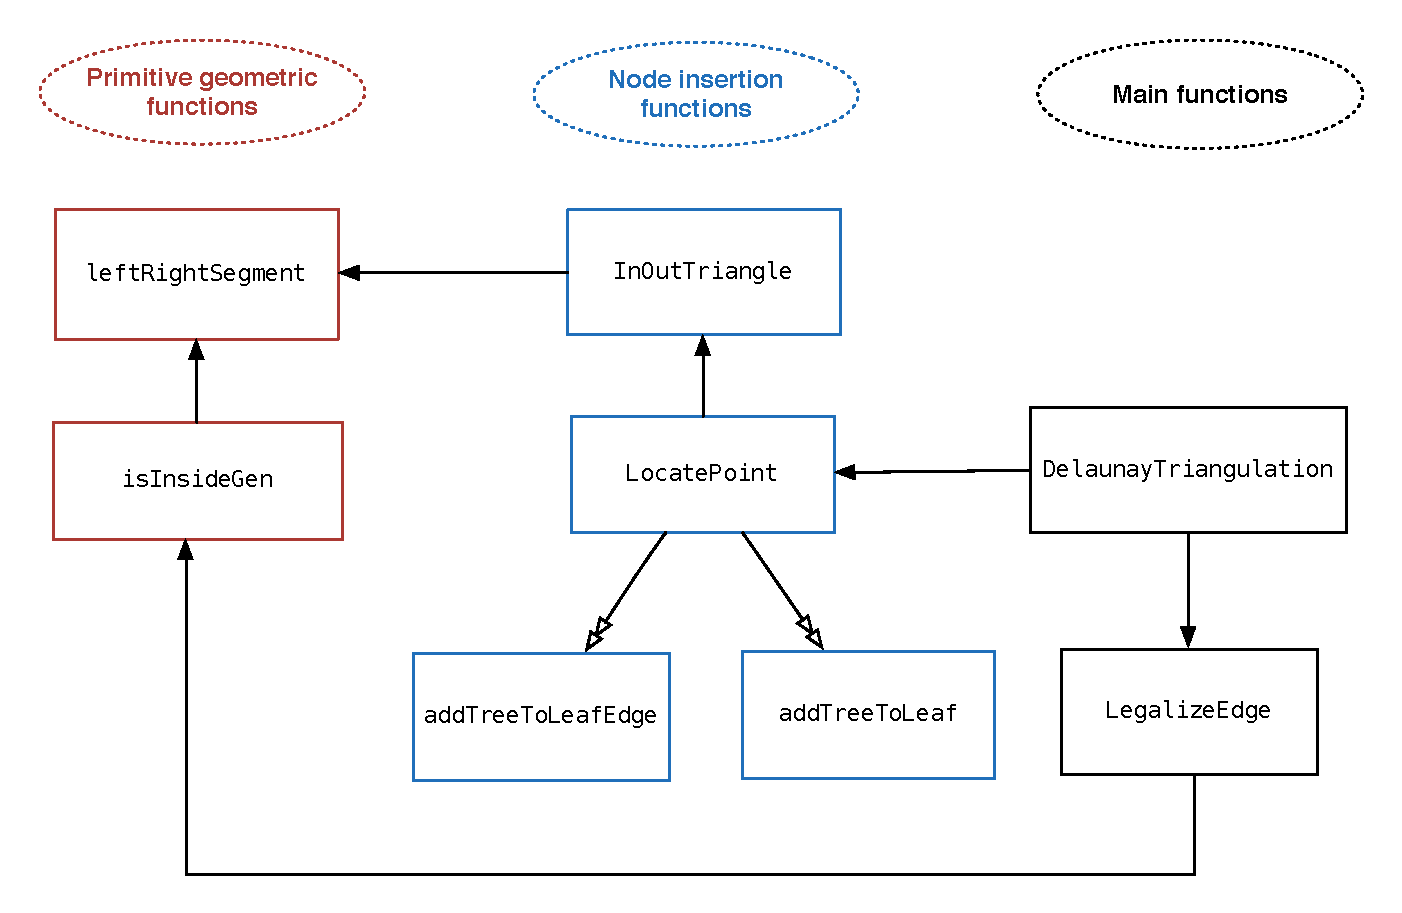
\includegraphics[width=0.8\textwidth]{images/Prog.eps}
\caption{Main architecture of the code. The simple arrows mean "use this function" and the double arrows mean "have as consequences".}
\label{fig:progArchitecture}
\end{figure}

Figure \ref{fig:progArchitecture} depicts the global architecture of our code. We have basically 4 types of functions : 
\begin{itemize}
\item the primitive \textbf{geometric functions} : 
\begin{enumerate}
\item \texttt{leftRightSegment} test whether a point lies on the right or on the left of a segment;
\item \texttt{isInsideGen} test whether a point lies inside or outside of a circle (it calls \texttt{leftRightSegment} because we need to have an oriented circle).
\end{enumerate}
It is important to notice that even if these functions seem trivial, they are the core of our code which determine the correctness of the code as we base all our processes on the answer of these functions. These are the only functions where we actually make computation (see section "Robustness" for more informations).
\item the \textbf{insertion functions} which performs 
\begin{enumerate}
\item the localisation step (the critical operation is \texttt{leftRightSegment} which is required to know in which triangle the adding point is);
\item the adding step : it adds it to the tree structure. This ere mainly manipulate pointer and create new structure's elements.
\end{enumerate}
\item the \textbf{main functions} : 
\begin{enumerate}
\item \texttt{DelaunayTriangulation} which is the main function performing the Delaunay's triangulation;
\item \texttt{LegalizeEdge} which performs the pivot operation (the critical operation is \texttt{isInsideGen} which determine whether the pivot is performed or not).
\end{enumerate} 
\item the \textbf{maintenance functions} (useful but not interesting function, which is why they are not figured on figure \ref{fig:progArchitecture}) : 
\begin{enumerate}
\item the functions to create the structures (\texttt{meshPointCreate}, \texttt{meshEdgeCreate}...).
\item the stack functions useful to manipulate the stack (\texttt{DeleteStackElement}...)
\end{enumerate}
\item the graphical interface functions (in \texttt{glfem.c}).
\end{itemize}
\section{Robustness}
\section{Performances results}



\begin{figure}
\centering 
\begin{subfigure}[b]{0.4\textwidth}
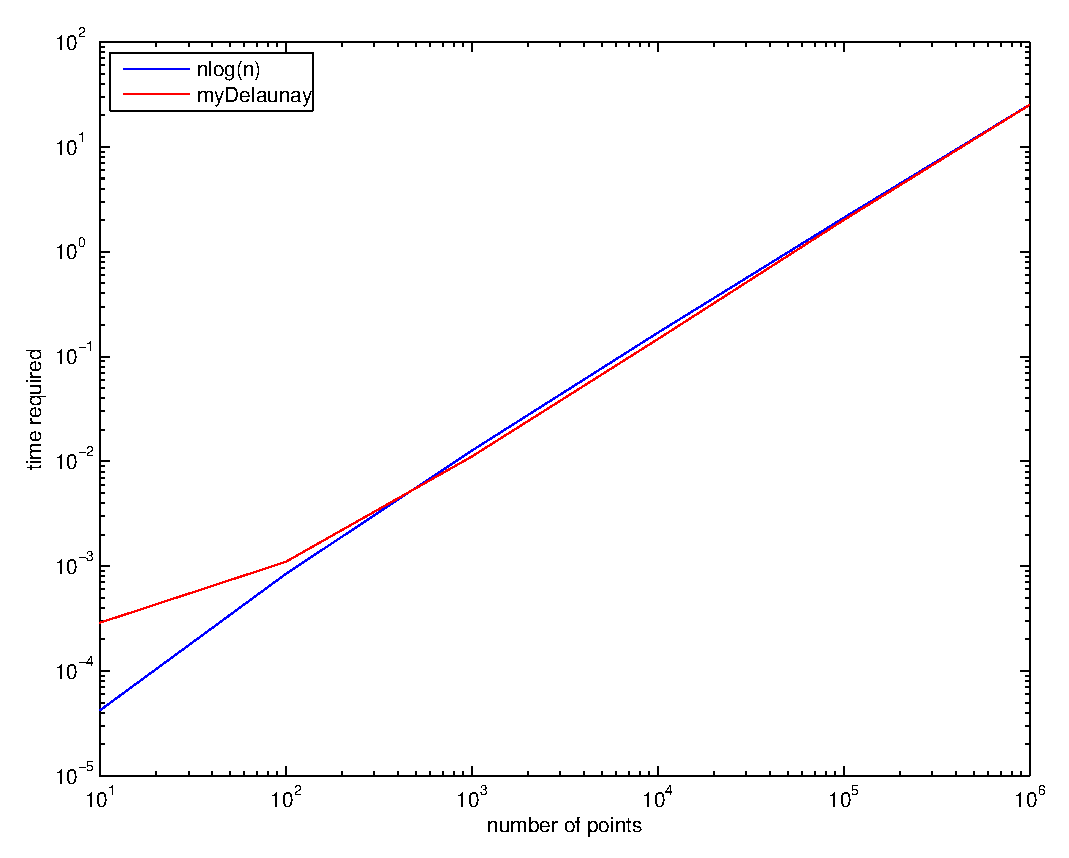
\includegraphics[width=\textwidth]{images/timeRandom.eps}
\caption{Computation time (red line) for points from $1e1$ to $1e6$ randomly choosen and theoretical time (blue line) $n\log n$.}
\label{fig:timeRandom}
\end{subfigure}
~
\begin{subfigure}[b]{0.4\textwidth}
\includegraphics[width=\textwidth]{images/timeLimit.eps}
\caption{Computation time (red line) for points from $1e1$ to $1e5$ randomly choosen and theoretical time (blue line) $n^2$.}
\label{fig:timeLimit}
\end{subfigure}
\end{figure}


 0.9903    0.6364    0.6458    0.8147    0.7976    0.8054

\newpage
\bibliographystyle{plain}
\bibliography{biblio.bib}

\end{document}